\documentclass[11pt]{amsart}
%%% WARNING: Do NOT change the page size, fonts, or margins!  Penalties will apply.


\usepackage{graphicx, hyperref}
\usepackage{amssymb,amsmath,amsthm, mathtools}
\usepackage{placeins} %enables \FloatBarrier, that prevents floats from going below it.
\usepackage{caption}
\usepackage{subcaption}
\usepackage{algpseudocode, algorithm}
\usepackage{tikz}
\usepackage{physics}
\usetikzlibrary{arrows}
\usetikzlibrary{tikzmark}

%%% WARNING: Do NOT change the page size, fonts, or margins!  Penalties will apply.
%%% WARNING: Do NOT change the page size, fonts, or margins!  Penalties will apply.

% Some macros for ease of use
\newcommand{\R}{{\mathbb R}}
\newcommand{\A}{{\mathrm{A}}}


\begin{document}

\title{Angle approximation from pressure measurements}
\author{Cannon Tuttle, Curtis Evans, Spencer Ashton, Tyler Sanders}

%% comment out next command to put today's date after names of group members, or put a desired day in the parethesis
\date{}

\maketitle

\begin{abstract}
    
\end{abstract}

%% First Section
\section{Problem Statement and Motivation}
A BYU Acoustics Research Group project is currently using a microphone array and triangulation to calculate the direction of arrival of a 
source in relation to the center of the array. They’ve implemented some rudimentary filtering, but so far the results of the calculation are 
somewhat unreliable. We want to take this process and model it as a time series/Hidden Markov model in order to optimize the calculation process. 
We will potentially employ Kalman filtering in order to filter angle measurements. We will also explore whether cross-correlation or GCC-PHAT 
is the better measure of coherence between microphone signals for this purpose, and whether the hidden state should be modeled as an angle or 
be modeled directly as a series of coherence measurements. We will also experiment with ways to represent the observation space. This will also 
include trying to predict whether there is or isn’t a speaker currently present.


Several of the noise reduction algorithms they have implemented depend on a highly accurate angle measurement. As those algorithms have already been 
implemented, we would be primarily concerned with the step of direction of arrival angle estimation and optimization, as well as optimally estimating 
the corresponding time delay. This would provide the research group with enhanced measurements for use in their noise processing algorithms.
	

This relates to the hidden markov model because we don’t know what the angles are that we are looking for, but we do know how to take a measurement of 
the current pressure at each microphone. We will use these microphones to be our observed data to then figure out what these angles are by creating a HMM. 
The angles are to be calculated at discrete time steps according to the current pressure measurement. The Kalman filter might accurately represent the 
system and more optimally combine current and prior information about the angle in order to calculate a less noisy current angle estimate.

%% Second Section
\section{Data}
The data for this project will be provided by the research team (Curtis Garner) that is currently working on it. The data includes measurements where the sound 
source is and is not moving, is and is not present, and measurements that do and don’t include machine noise in the microphone signal.




%% Third Section 
\section{Methods}
We have tried several methods to compute the hidden angle measurement. We tried the following methods...

\subsection{State Space Model}
First we had to set up our continuous state space model. We needed angular velocity in our state space so to do that we do a finite difference approximation 
where $\theta'_t \approx \frac{\theta - \theta_{t-1}}{\Delta t}$. Now that we have angular velocity we can use it to make a simple forward Euler step in our state 
space. With the finite difference we need to save $\theta_{t-1}$ in the state space. This yields the following setup
\[\mathbf{x}_t = \begin{pmatrix*}[l]
    \theta_t \\
    \theta_{t-1} \\
    \theta'
\end{pmatrix*},\;  
F = \begin{pmatrix*}[l]
    1 & 0 & \Delta t \\
    1 & 0 & 0 \\
    \frac{1}{\Delta t} & \frac{1}{\Delta t} & 0
\end{pmatrix*},\;
H = \begin{pmatrix*}[l]
    1 & 0 & 0 \\
    \vdots & \vdots & \vdots\\
    1 & 0 & 0

\end{pmatrix*}\]
 where $H$ is of dimension $n\times3$ for $n$ observed angles. We don't have any control in our situation so our state space is
 \[\mathbf{x}_t = F\mathbf{x}_{t-1} + \mathbf{w}_t,\]
\[\mathbf{z}_t = H\mathbf{x}_t + \mathbf{v}_t\].

\subsection{Kalman Filter}
We implemented the Kalman filter from the Volume 3 Textbook \cite{V3}. To understand how angle measurements worked in the Kalman Filter we tried it with
stimulated data done in the lab manuals and class. We discovered a problem with the update step in angle wraparound from the angles in the range of 
\[2\pi - \epsilon \leq \theta \leq 2\pi + \epsilon\] for some $\epsilon \geq 0$. We notices that the more noise we added the larged this $\epsilon$ got. 
See figure \ref{fig:simple_kalman} to get a visual.

We discovered that the problem was occurring in the update step where \[\mathbf{\tilde{y}}_k = \mathbf{z}_k - H\mathbf{\hat{x}}_{k|k-1}.\]
A toy example would be if we are looking at an observed angle $\mathbf{z}_i = 15^{\circ}$ and a predicted angle of $(H\mathbf{x})_i = 355^{\circ}$ 
then $\mathbf{z}_i - (H\mathbf{x})_i = 15^{\circ} - 355^{\circ} = -340^{\circ}$ and we desire $20^{\circ}$. We could simply do this by noticing that $-340 \equiv 20 \pmod {360}$,
however, if we said $\mathbf{z}_i=355^{\circ}$ and $(H\mathbf{x})_i = 15^{\circ}$ then $\mathbf{z}_i - (H\mathbf{x})_i = 355^{\circ} - 15^{\circ} = 340^{\circ}$ which isn't what we want.
We want the Kalman filter to think of this difference as $-20^{\circ}$. The best way to do this was by implementing Algorithm \ref{alg:kalman} which will get us the right differenced needed by 
the correct sign so the Kalman filter can function correctly.

\begin{figure}[htp]
    \centering
    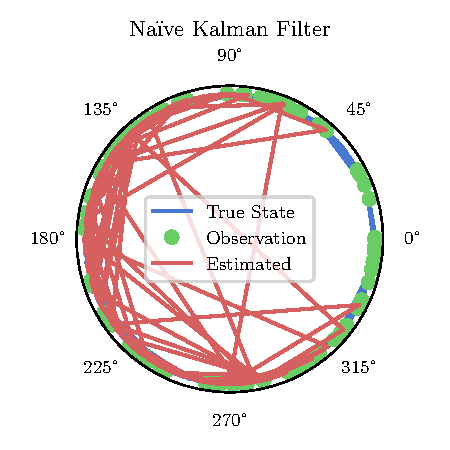
\includegraphics[width=0.47\textwidth]{non_altered_kalman.pdf}\hfill
    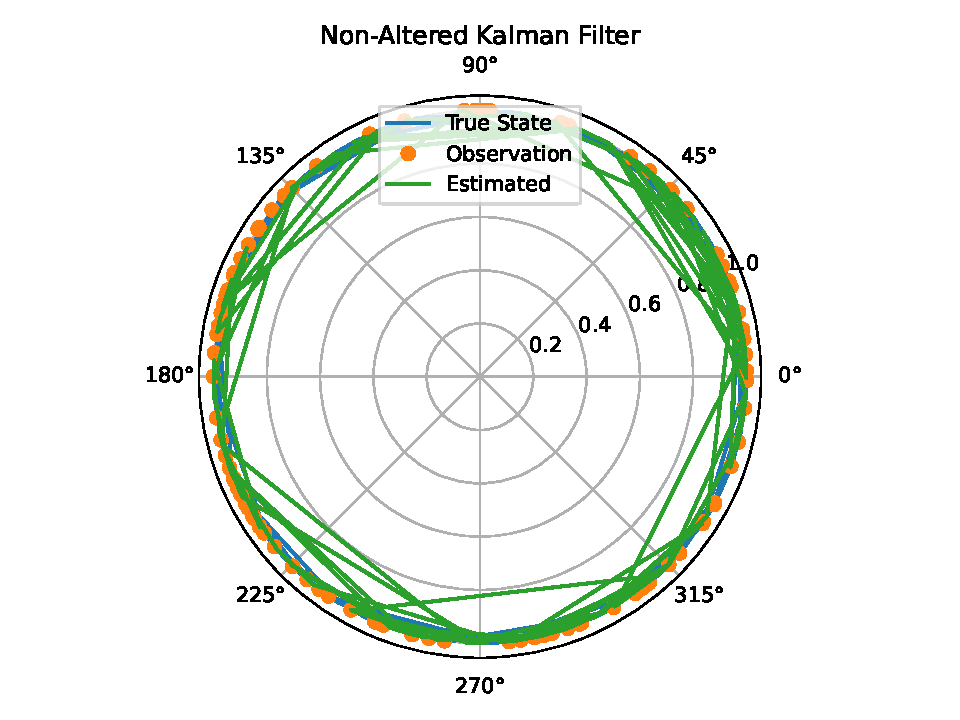
\includegraphics[width=0.47\textwidth]{altered_kalman.pdf}\hfill
    \caption{The non-altered and altered Kalman Filter}
    \label{fig:simple_kalman}
\end{figure}



\begin{algorithm}
    \caption{Process to Fix Wraparound}\label{alg:kalman}    
    \begin{algorithmic}
        \State $\mathbf{v} \gets \mathbf{z}_t - H\mathbf{x}_t$
        \If{$\lvert{\mathbf{v}}\rvert \geq \pi \;\textbf{and}\; \mathbf{v}\leq 0$} 
            \State $\mathbf{v} \gets \mathbf{v} + 2\pi$
        \ElsIf{$\lvert{\mathbf{v}}\rvert \geq \pi \;\textbf{and}\; \mathbf{v} \geq 0$} 
            \State $\mathbf{v} \gets \mathbf{v} - 2\pi$
        \EndIf 
        \State $\tilde{\mathbf{y}_t} = \mathbf{v}$ 
        \end{algorithmic}
    \end{algorithm}

%% Insert some pictures of the angle adjustment and add the algorithm 

\subsection{Particle Filter}

TODO graph of Von Mises distribution with explanation of how Kappa parameter 
correlates to certainty on particle's location.

TODO explain basis principles of Particle Filter and cite the book
that Tyler referenced in implementation.

\subsection{Leaky Filter}

TODO explain leaky filter and how it is working

\section{Results}

We had success with circular filtering techniques by using Algorithm \ref{alg:kalman} allowed us to use Kalman Filters with circular mechanics.


\section{Analysis}

TODO tradeoffs of Particle filter - the compute time 500x longer for 500 particles
- particle filter can have a more flexible prior because it's already got particles everywhere.
- particle filter better at nonlinearities bc particles can be reassigned

- Both systems have a mechanism to capture how certain they are about the current state,
- and both have a way to specify how much we "belive" current measurements

\section{Ethical Considerations}
This project seeks to augment the safety of those outside the machinery by increasing the awareness of the machine operators. However, before deployment, this model must be 
shown to improve safety as much as or more than it increased the safety perception of the operators. Risk compensation “is a theory which suggests that people typically adjust 
their behavior in response to perceived levels of risk, becoming more careful where they sense greater risk and less careful if they feel more protected” [citation]. This should 
be accounted for before deploying these methods in the field to ensure that the model performs robustly enough to truly enhance overall safety, despite risk compensation. Furthermore, 
it should be emphasized that operators should still use sight and radio communication to identify nearby individuals, and that people near machinery must still exercise caution. 

\section{Conclusion}













\begin{figure}[htp]
    \centering
    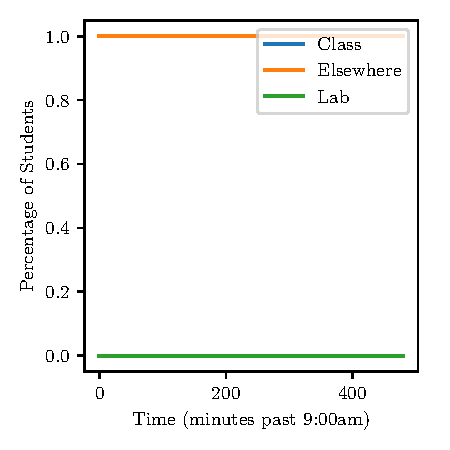
\includegraphics[width=0.45\textwidth]{temp.pdf}\hfill
    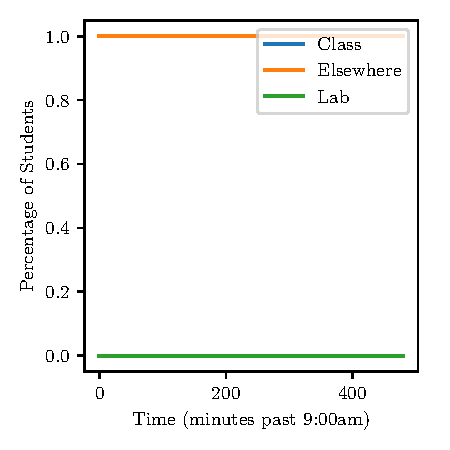
\includegraphics[width=0.45\textwidth]{temp.pdf}\hfill
    \caption{The constant alpha functions (left) along with the timeplot using IVP (right).}
    \label{fig:constant_alpha}

\end{figure}


\begin{figure}[htp]
    \centering
    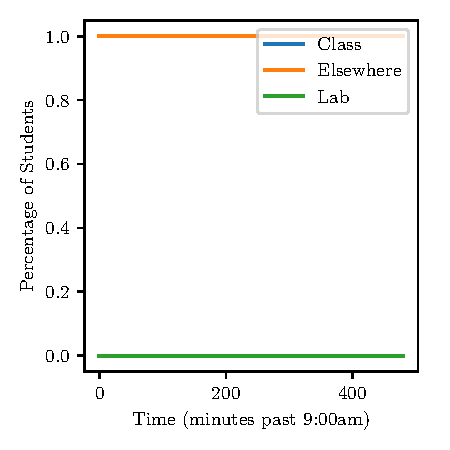
\includegraphics[width=0.45\textwidth]{temp.pdf}\hfill
    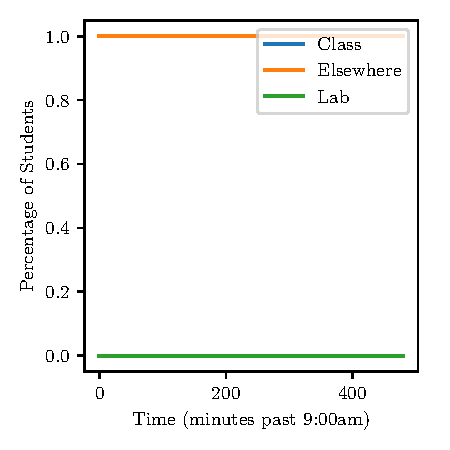
\includegraphics[width=0.45\textwidth]{temp.pdf}\hfill

    \caption{The discontinuous alpha functions (left) along with the timeplot using IVP (right).}
    \label{fig:discontinuous_alpha}

\end{figure}




\begin{figure}[htp]
    \centering
    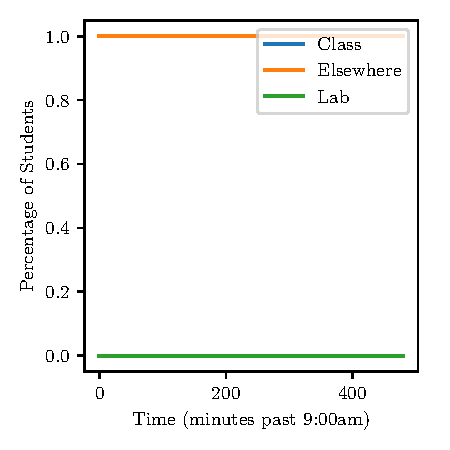
\includegraphics[width=0.3\textwidth]{temp.pdf}\hfill
    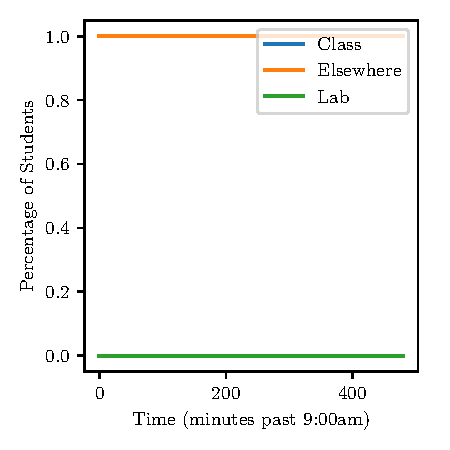
\includegraphics[width=0.3\textwidth]{temp.pdf}\hfill
    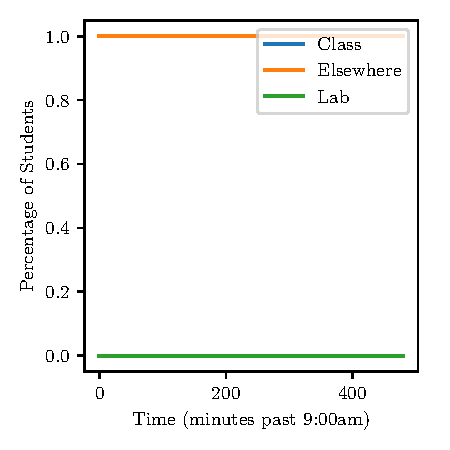
\includegraphics[width=0.3\textwidth]{temp.pdf}\hfill
    \caption{Simulating with $A_{interp.12}$ (left), giving the timeplots using both IVP (center) and BVP (right).}
    \label{fig:continuous_alpha}

\end{figure}









%%%%%%%%%%%%%%%%%%%%%%%%%%%%%%%%%%%%%
%% Bibliography below
%%%%%%%%%%%%%%%%%%%%%%%%%%%%%%%%%%%%%
\FloatBarrier % Keep the figures from being put after the bibliography
\newpage
%% If using bibtex, leave this uncommented
%\bibliography{refs} %if using bibtex, call your bibtex file refs.bib
\bibliographystyle{alpha}

%% If not using bibtex, comment out the previous two lines and uncomment those below
\begin{thebibliography}{99}
\bibitem{V3} The ACME Volume 3 Textbook
\bibitem{Particle} Labbe, Roger. “Kalman and Bayesian Filters in Python”.
\bibitem{Population} Pierre Auger, Jean-Christophe Poggiale, Emergence of Population Growth Models: Fast Migration and Slow Growth, Journal of Theoretical Biology, Volume 182, Issue 2, 1996, Pages 99-108, ISSN 0022-5193, https://doi.org/10.1006/jtbi.1996.0145.
\end{thebibliography}

\end{document}
